\section{Grundlagen}
\label{section:grundlagen}

\subsection{Threads in Java}
\label{sections:treads_prozesse}
Java-Threads werdem vom Betriebssystem verwaltet, sog. \textit{native threads} oder auch \textit{kernel threads}.
Hierbei wird die Steuerung der Ausführungsreihenfolge, die Zuweisung der Rechenzeit und der Prozess- \& Threadwechsel
vom Scheduler \& Dispatcher des Betriebssystems übernommen\parencite[Kapitel 2]{Tanenbaum2016}.
Die Threading-Abstraktion in Java bietet Entwicklern verhältnismäßig leichten Zugriff auf parallelle Programmierung und Synchronisation von Threads.
Servlet-Container binden üblicherweise jede vom Webserver weitergeleitete Anfrage an einen
Thread\footnote{Aus einem, im vornherein erzeugten, Thread-Pool} im Servlet-API, welcher die jeweilige Anfrage imperativ abarbeitet
(daher auch \textit{worker thread} bezeichnet).
Der auszuführende Code ist in diesem Ansatz an den jeweiligen Thread gekoppelt. Sobald im Code ein asynchrones Ereignis aufgerufen wird
, wird die weitere Abarbeitung der Instruktionen vom Thread blockiert, bis es abgeschlossen ist.

\noindent
Um jede Anfrage, und somit jeden Thread, möglichst parallel zu bearbeiten wird vom Scheduler
des Betriebssystems für jeden Prozessorkern regelmäßig ein Kontextwechsel zwischen den Threads,
ein \textit{Threadwechsel} (\textit{thread-switch}), veranlasst.
Der Dispatcher entzieht dabei dem derzeit aktiven Thread die CPU und teilt sie anschließend dem nächsten Thread zu.

Während bei einem Kontextwechsel von Prozessen (Prozesswechsel) der gesamte Programmkontext (Adressräume, Inhalt der CPU-Register,
Seitentabelle, geöffnete Dateien und Metainformationen)
gewechselt werden muss, wird bei einem Threadwechsel lediglich der Inhalt der CPU-Register (inkl. Programmzähler)
ersetzt\parencite{Brosenne2021}\parencite{Mosberger2002}.

\noindent
Da der Threadwechsel, im Fall von \textit{kernel threads}, durch Systemaufrufe, also vom Kernel des Betriebssystems, ausgeführt werden muss, entsteht
bei einem Threadwechsel dennoch ein messbarer Zeitverlust.
Dies ist durch die geringe Geschwindigkeit und den Overhead des notwendigen Softwareinterrupts bedingt.
Der Softwareinterrupt erfolgt, um die Programmausführung im Benutzer-Modus zu unterbrechen und die Ausführung des Interrupt-Handlers im
Kernel-Modus (Kontextwechsel auf privilegierten Ring 0) zu erzwingen , sowie auf dessen Beendigung zu warten.
Weitere Threadwechsel entstehen, wenn ein Thread die zugewiesene Rechenzeit nicht nutzen kann, da er noch durch eine I/O-Operation
blockiert, und diese vom Scheduler einem anderen Thread zugeteilt werden muss.

\noindent
Bei Client-Server Kommunikation kann das Blockieren einer I/O-Operation zwei Gründe haben:
\begin{enumerate}
	\item Eine Lese-Operation wartet auf Daten, die über das Netzwerk transportiert werden
	\item Eine Schreib-Operation muss warten bis die Puffer des Ziels (wieder) aufnahmebereit sind
\end{enumerate}

\noindent
Während die Kosten von Threadwechseln für, nach früheren Standards, hoch frequentierte Anwendungen lange Zeit kein Problem darstellte,
sind die Anforderungen an Webanwendungen in den letzten Jahren durch steigende Nutzerzahlen und Architekturen,
die stark auf Client-Server-Kommunikation basieren, wie Microservices und SPAs, erheblich gestiegen.

\noindent
Sobald die Last eine realistische, kritische Grenze erreicht, erfolgen die Threadwechsel zwischen \textit{kernel threads} vom Betriebssystem
nicht mehr schnell genug, um jede Anfrage innerhalb einer akzeptablen Zeit zu bearbeiten bzw. jedem Thread ausreichend Rechenzeit zuzuweisen.
Die Kosten der Threadwechsel von \textit{kernel threads} können also zu einem Performance Problem führen, welches sich in nicht
ausreichend skalierendem Durchsatz äußert.

\subsection{Reaktive Programmierung}
\label{section:reaktive_programmierung}
Reaktive Programmierung ist ein Programmierparadigma, bei dem der Programmablauf als Sequenz von asynchronen Ereignissen (Events), und
Daten als, von außen unveränderliche (immutable), Datenströme (Streams) dargestellt werden.
Sobald es innerhalb des Datenstroms zu Änderungen kommt werden diese als Events durch einen Publisher veröffentlicht.
Diese Events werden dann von einem oder mehreren \verb|Subscribern| konsumiert. Diese können wiederrum weitere Events durch einen Publisher veröffentlichen.

Die treibende Kraft bzw. der Stimulus von reaktiven Anwendungen sind also interne Änderungen innerhalb der Datenströme, wie beispielsweise das
Hinzufügen eines Elements, welche anschließend den weiteren Programmablauf durch das Auslösen eines Events (durch einen Publisher) starten.

Die Grundidee orientiert sich am Observer-Pattern und dessen Ausprägung dem Publish-Subscribe Pattern, erweitert diese aber
noch um die Benachrichtigungen des Subscribers:
\begin{enumerate}
	\item Sobald keine Events mehr kommen
	\item Wenn ein Fehler aufgetreten ist
\end{enumerate}
Indem Änderungen eines Datenstroms direkt propagiert werden und der Subscriber diesen nicht modifizieren kann, sondern lediglich über Änderungen informiert wird,
können Programme ohne jeglichen Zustand realisiert werden\parencite{Escoffier2017}.

Während ein Datenstrom selber von außen unverändlich ist, kann aber dennoch der Inhalt, also die Daten,
des vom Publisher veröffentlichten Events modifiziert werden, bis es vom
Subscriber konsumiert wird, und zwar in beliebig vielen Schritten.

Für eine solche Verkettung von Verarbeitungsschritten für Events bzw. Daten
wird oft der Begriff \verb|Pipeline| verwendet und jeder Verarbeitungsschritt als \verb|Pipe| bezeichnet.
Durch diese Pipelines \textit{fließen} Elemente in Form von Events bzw. Daten von ihrer Quelle
bis zu einer Senke, dem Ziel bzw. dem eigentlichen Subscriber der \verb|Pipeline|.

Daher wird dieser Prozess auch als \verb|event flow| oder \verb|data flow| bezeichnet.
Jede \verb|Pipe| kann ein Element ändern, löschen oder auch neue Elemente erstellen und dem \verb|flow| hinzufügen.

Allgemein fließt ein Element immer stromabwärts also von der Quelle zur Senke
\footnote{Es gibt aber auch Ausnamefälle in denen ein Element stromaufwärts fließt, also von einer pipe oder von der Senke zur Quelle},
dabei wird die vorherige \verb|pipe| als \verb|upstream| bezeichnet und die nächste, zu durchfließende \verb|pipe| als \verb|downstream|.
Im Hintergrund kommt dabei wieder das Publish-Subscribe Pattern zum Einsatz. Elemente werden von einer durchlaufenen \verb|pipe| durch \verb|Publisher|
veröffentlicht und von der nächsten \verb|pipe| als \verb|Subscriber| konsumiert.

Jede \verb|Pipe| kann eine Vielzahl an konkreten Operatoren enthalten die in der jeweiligen Reactive Programming-Bibliothek definiert sind.
\footnote{Obwohl die Implementierungsdetails und die verwendete Terminologie unterschiedlich, abhängig von der verwendeten Reactive Programming-Bibliothek
	und der Programmiersprache, sind, ist der Arbeitsablauf immer ähnlich}
In Listing \ref{lst:eventflow_pseudocode} wird der Event-/Datenfluss anhnd von Pseudocode dargestellt und in Abbildung \ref{fig:eventflow_mutiny}
wird der typische EventFlow in der Reactive Programming-Bibliothek \verb|Mutiny| dargestellt.
\begin{lstlisting}[caption=Pseudocode Event-/Datenfluss, captionpos=b, label=lst:eventflow_pseudocode]
source <-- source ist der Beginn des streams, also die Quelle
	.operator1()  <-- operator1 nimmt die Elemente des Upstreams(source) entgegen, modifiziert diese und gibt sie an den Downstream(operator2()) weiter
	.operator2()  <-- operator2 nimmt die Elemente des Upstreams(operator1()) entgegen, modifiziert diese und gibt sie an den Downstream(consumer) weiter
	.subscribe(consumer) <-- consumer ist das Ende des Streams, also die Senke
\end{lstlisting}

\begin{figure}[h!]
	\centering
	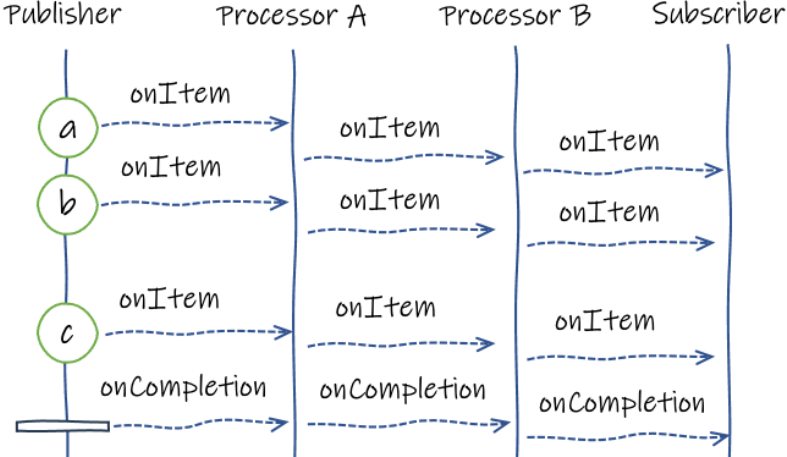
\includegraphics[width=0.8\textwidth]{EventFlow}
	\caption{Exemplarische Abbildung eines Event Flow in der Reactive Programming-Bibliothek Mutiny \parencite{MutinyEventFlow}}
	\label{fig:eventflow_mutiny}
\end{figure}

Reaktive Programmierung verinnerlicht das Konzept von nicht-blockierender bzw. asynchroner Ein- und Ausgabe (I/O).
Dabei wird, statt wie bei synchroner bzw. blockierender Ein- und Ausgabe die restliche Ausführung des Programms
zu blockieren bis die Datenübertragung abgeschlossen ist, nach dem Start der Übertragung bereits begonnen die Teile des
Programms auszuführen, die nicht von dem Ergebnis der I/O Operation abhängen.

\begin{lstlisting}[caption=Pseudocode Nonblocking I/O (NIO), captionpos=b, label=lst:NIO_Pseudocode]
	NonBlockingDatabaseRequest()
		.subscribe(print("req finished"))
	NonBlockingDatabaseRequest2()
		.subscribe(print("req 2 finished"))
	print("hello world")
\end{lstlisting}
In \ref{lst:NIO_Pseudocode} kann durchaus zuerst \verb|hello world| ausgegeben werden, da die gestarteten Datenbank-Anfragen die
restliche Programmausführung nicht blockieren. Wenn statt \verb|hello world| versucht würde, die Ergebnisse einer der Datenbank-Abfragen
darzustellen wäre das Ergebnis in der Regel eine Exception oder \verb|null|, da die Anfragen zur Zeit der Ausführung von Zeile 5 noch nicht notwendigerweise
abgeschlossen sind. Das ist ein sehr weit verbreiter Fehler beim Arbeiten mit asynchronen, nicht-blockierenden I/O-Operationen.

Methoden die blockierende I/O Operationen ausführen, wie Datenbankzugriffe oder Anfragen von externen Services,
geben beim Aufruf unverzüglich einen Publisher zurück, auf dem sich der Aufrufer als \verb|Subscriber| registriert.
Dadurch wird der bearbeitende Thread nicht blockiert, und kann die nächste Anfrage bearbeiten.
Sobald das Ergebnis der I/O Operation bereit ist, wird es dem Publisher in Form eines Events mitgeteilt, von diesem veröffentlicht und die Anfrage kann
vom Aufrufer bzw. Subscriber weiter bearbeitet werden.
Da durch dieses Modell der auszuführende Code nicht mehr an den jeweils ausführenden Thread gebunden wird, erlaubt es die Nutzung eines einzigen
Threads (\textit{sog. IO Thread}) statt eines \textit{Threadpools} für die Verarbeitung von vielen Anfragen.

\subsubsection{Vorteile und Nachteile}
\label{section:vorteile_nachteile}

Die Vorteile der Nutzung von einigen wenigen \verb|kernel threads| als \verb|IO Threads| gegenüber eines ganzen Threadpools
an \verb|kernel threads| liegen insbesondere in den Antwortszeiten bei hoher Last und dem Ressourcenverbrauch.
Umso weniger \verb|kernel threads| gleichzeitig aktiv sind, umso weniger Threadwechsel gibt es auch pro CPU-Kern, wodurch die Antwortzeiten von Anwendungen
wesentlich besser mit der Erhöhung der Last skalieren können, da Threadwechsel nicht mehr der limitierende Faktor sind.
Darüber hinaus sinkt dadurch auch der allokierte Speicher deutlich
\footnote{Eine 64Bit-JVM reserviert auf Linux-und Solaris-Systemen standardmäßig 1 MB Speicher für den Threadstack eines Threads}
und der Grad der Parallellität wird nicht mehr von der Anzahl der verfübaren Threads begrenzt.

Die Umstellung auf das reaktive Programmierparadigma erfordert allerdings eine Änderung in der Denk- und Herangehensweise in der
Entwicklung von Softwarekomponenten. Denn reaktive Komponenten haben in der Regel keinen Zustand,
sondern reagieren lediglich auf interne Änderungen in den zugrundeliegenden Datenströmen.
Die bisherigen Programmabläufe müssten daher als reaktive Pipelines neu konstruiert werden.

Darüber hinaus ist reaktiver Code schwieriger zu debuggen und zu testen als imperativer Code, denn die Programmlogik die in den einzelnen Operatoren
der \verb|Pipes| einer \verb|Pipeline| aufgerufen wird, besteht aus anynomen Funktionen.
Während \verb|Event Flows| bei kleinen Pipelines noch zu überblicken sind, können komplexe Pipelines, die sich über die ganze Anwendung erstrecken,
außerdem, schnell unklar werden.

//schwer zu lernen da soviele anbieter mit verschh. nomenklaturen und ansätzen, wie RxJava mit dem (FRP ansatz), kaum bis keine gute fachliteratur
//integration in bestehende enterprise anwendungen schwer da jede schicht reactiv sein muss und transaktionen, security datenbanktreiber noch an
thread gebunden -> hier muss jede schicht reaktiv werden bzw. jedes framework oder bibliothek
//TODO: mehr als nur stichpunkte (abschließend nochmal in stichpunkte?)
//Da nur ein IO-Thread genutzt wird resultieren blockierende I/O-Operationen in der Blockierung der gesamten Anwendung

Allerdings gibt es auch einige gravierende Nachteile:

\begin{enumerate}
	\item Asynchroner Code ist schwieriger zu schreiben, lesen, testen und zu debuggen als imperativer Code
	      //TODO:  Warum? Anderes Paradigma, anonyme Funktionen (stacktrace schwierig)
	\item Durch Vielzahl an Anbietern die (bis Java 9) keine gemeinsame Basis hatten ist die Nomenklatur extrem umfangreich und uneindeutig und die grundlegenden
	\item Heransweise unterschiedlich bspw. RxJava nutzt Observables (erweitert das Observer Pattern), Unterschiedliche Klassennamen und
	      Anzahl an Operatoren (RxJava über 50)
	\item Verwechslung mit ähnlichen Begriffen wie Functional Reactive Programming (RxJava) die Operatoren wie .map oder .filter nutzen

	\item Sehr aufwendig in bestehende klassische Anwendungen zu integrieren //TODO:  Warum? Da jede Schicht reaktiv sein muss
	      und klassische Enterprise Anwendungen
	\item bzgl Security oder Transaktionen immer noch an einen Thread gebunden sind
	\item ges—the callbacks or combinators—are anonymous, i.e. not addressable.
	      This means that they usually handle success or failure directly without signaling it to the outside world. This lack of addressability makes recovery
	      of individual stages harder to achieve as it is typically unclear where exceptions should, or even could, be propagated.
	\item Reaktive Anwendungen müssen in jeder Schicht reaktiv sein (Transaktionen, Security, Datenbanktreiber) und daher schwer in klassische Anwendungen
	\item zu integrieren, besonders ohne Dispatching Mechanismus (wenn blockierender Endpunkt -> Code auf Worker-Pool ansonsten IO-Thread)
	\item Da nur ein IO-Thread genutzt wird resultieren blockierende I/O-Operationen in der Blockierung der gesamten Anwendung
\end{enumerate}


\subsubsection{Alternativen}
In Java 1.1 wurden Threads als sog. \textit{Green Threads} implementiert. Dabei wurde die Möglichkeit Threads vom Betriebssystem verwalten zu lassen
gar nicht genutzt. Stattdessen lief die komplette JVM in einem einzigen Prozess //TODO: eigentlich Thread oder ?.
\textit{Green threads} waren als \textit{user threads} implementiert \footnote{Auch als \textit{Fiber} oder \textit{virtual thread} bezeichnet},
dabei ist die Funktionalität
nicht im Kernel implementiert (wie bei \textit{kernel-/native threads}), sondern in einer Programmbibliothek im \textit{Userspace}.
Da sich das Betriebssystem nicht um das Scheduling von \textit{user threads} kümmert, wurde dies über einen eigenen Scheduling-Algorithmus der JVM
geregelt.\parencite{Oracle2010}
Ein \textit{green thread} existiert lediglich als Objekt innerhalb der JVM, und durch die virtuelle Speicherverwaltung entfallen somit
die aufwändigen Betriebssystemaufrufe beim
Erstellen eines Threads, sowie bei Thread- bzw. Kontextwechseln, denn der ausführende Main-Thread bleibt gleich.

Die Threadwechsel der \textit{user-threads} erfolgten ausschließlich innerhalb des Main-Threads, weswegen keine echte Parallelität realisiert werden konnte,
da immer nur ein Prozessorkern genutzt wurde.
Während der Vorteil dieses Modells darin lag, dass es keine 'echten' parallelen Zugriffe auf eine Resource innerhalb des JVM-Prozesses geben konnte
und die Synchronisation von Datenzugriffen daher leicht war, überwog schließlich der Umstand, dass keine Nutzung von mehreren Prozessorkernen
durch Multithreading möglich war, weswegen \textit{Green Threads} ab Java 1.3 zugunsten von \textit{native threads} entfernt wurden.

Mit dem OpenJDK Projekt \textit{Project Loom} ist die Idee von \textit{Green threads}
wieder aufgegriffen worden, allerdings nun als Ergänzung (statt Alternative) zu \textit{native threads}.
Statt alle virtuellen Threads auf dem nativen Main-Thread auszuführen, werden diese von einer geringen Anzahl an nativen \textit{worker threads},
die als Carrier eingesetzt werden, ausgeführt.
Deren Anzahl ist so gewählt, dass alle CPU Kerne durch Multithreading dauerhaft benutzt werden können
\footnote{In der Praxis laufen natürlich noch andere Prozesse auf dem Server, deren Threads auch ausgeführt werden müssen.}
, aber so wenig Kontextwechsel wie möglich ausgeführt werden müssen.
\parencite{Oracle2021} \footnote{Im Idealfall würde auf jedem CPU Kern ein \textit{worker thread} laufen,
	ohne jemals einen Thread- bzw. Kontextwechsel zu machen.}
Während ein nativer Thread in einer 64 Bit JVM auf Linux-Systemen standardmäßig 1 MB für den Threadstack reserviert
und zusätzlich noch Metadaten abspeichert, ist ein virtueller Thread
lediglich ein Objekt im virtuellen Speicher der JVM und benötigt sehr wenig Resourcen (da er ja im Hintergrund von einem
nativen Thread abgearbeitet wird).
Aus diesem Grund können durchaus mehrere Millionen virtueller Threads erzeugt werden (bei entsprechendem allokierten Heap-Speicher der JVM), wohingegen
die Erstellung von 10.000 nativen Threads entweder den allokierten Speicher weit überschreitet (wodurch der JVM-Prozess abstürzt) oder die Threadgrenze
des Betriebssystems überschreitet.

Sobald ein virtueller Thread nun eine blockierende I/O Operation ausführt signalisiert er dem darunterliegenden nativen Thread, dass er momentan nichts machen
kann außer Warten, und erlaubt dem nativen Thread zu einem anderen virtuellen Thread zu wechseln.

Das große Versprechen des Projektes ist außerdem, das Entwickler keine asynchronen Programmierparadigmen (wie u.A. \textit{Reactive Programming})
nutzen müssen um die beschriebenen virtuellen Threads (und die damit einhergehenden wesentlichen Performanceverbesserungen) nutzen zu können.
Um dieses Versprechen zu halten werden virtuelle Threads, statt als Bibliothek eines Drittanbieters, in Form einer eigenen JDK Version bereitgestellt.
In dieser Version wurden viele Teile der Standardbibliothek die mit I/O-Operationen arbeiten so angepasst, dass virtuelle Threads statt native Threads
genutzt werden. Auf diese Weise können I/O-Operationen, wie beispielsweise der Aufruf einer Netzwerkfunktionalität, ohne Änderungen am Programm
die virtuellen Threads nutzen und blockieren den darunterliegenden nativen Thread nicht mehr.

\subsection{Reaktive Datenströme}
\label{section:reaktive_datenströme}
In einer typischen asynchronen Verarbeitungskette von, potenziell unbegrenzten, Datenströmen
bestehend aus einem Sender und Empfänger bzw. Publisher und Subscriber kann es vorkommen,
dass der Sender Daten schneller an den Empfänger verschickt, als dieser sie verarbeiten kann.
Zwei naive Ansätze mit einer Überlastung des Empfängers umzugehen wären:
\begin{enumerate}
	\item Nur der Empfänger reagiert auf eine Überlast. Diese kann sich in einem Speicherüberlauf äußern oder, falls der Puffer des Empfängers eine Größenbeschränkung
	      hat, im Verlust der empfangenen Daten
	\item Der Sender begrenzt im vornherein die Datenmenge, die er an den Empfänger schickt. Da der Sender allerdings in der Regel nicht weiß wieviel der Empfänger
	      verarbeiten kann, sendet er entweder zuviel (es entsteht eine Überlast), oder er sendet zuwenig wodurch der Durchsatz geringer ist als nötig
\end{enumerate}\parencite{JavaSpektrum2015}
Die Lösung für dieses Problem wird \textit{Backpressure} genannt.
Dabei fordert der Empfänger die Daten entsprechend seiner Kapazitäten an, wodurch der Sender weiß wieviele Daten er maximal versenden darf.
Diese Mitteilung muss asynchron geschehen, da bei einer synchronen Kommunikation der Backpressure die Vorteile der asynchronen, reaktiven Datenverarbeitung
negiert würden.
Da große Anwendungen aus mehreren Schichten (bspw. Routing-Schicht, Persistenzschicht, Geschäftslogik) bestehen und somit zwischen
dem Sender und Empfänger mehrere Komponenten liegen können, muss jedes
Element der Verarbeitungskette nichtblockierendes, asynchrones Verhalten implementieren, da ansonsten der Rest der Kette blockiert würde.

Aus der Intention einen Standard für die asynchrone Verarbeitung von Datenströmen mit nicht-blockierender \textit{back pressure}
zu schaffen, ging die \textit{Reactive Streams}-Initiative hervor.
Innerhalb dieser Initiative haben sich mehrere Arbeitsgruppen gebildet, welche die grundlegenden Semantiken erarbeitet haben und
sie in Form einer eigenen Java-Spezifikation namens \textit{Reactive Streams}-API implementiert und veröffentlicht haben.\parencite{ReactiveStreams}
Diese API wurde anschließend in Java 9, als Schnittstelle namens \textit{Flow-API} dem JDK hinzugefügt.
Die \textit{Flow-API} des JDK entspricht der \textit{Reactive Streams} Spezifikation und stellt (nur) Interfaces zur Verfügung mit denen eine
asynchrone, nicht blockierende Verarbeitung von (unbegrenzten) Datenströmen mit \textit{back pressure} auf der JVM implementiert werden kann.
\parencite{OracleFlow}.
\footnote{Nicht zu Verwechseln mit den Java-Streams durch die Collection-API ab Java 8. Diese sind zur Auswertungszeit in ihrer Größe begrenzt und
	nach der Abarbeitung liegt statt eines Streams eine Collection vor}
\subsubsection{Java Flow-API}
\label{section:java_flow_api}
//TODO: Erwähnen welche Klassen in API (pPublisher, Subscriber, Subscription und Processor)- FLow-Api als Subchapter erklären vllt mit Diagramm
//Und wie diese Backpressure eimplementieren durch den Zwischenschritt der Subscription
//When a Subscriber registers itself on a Publisher, the Publisher’s first action is to
invoke the onSubscribe method to pass back a Subscription object. The Subscription interface
declares two methods. The Subscriber can use the first method to notify the Publisher that it’s ready to process a
given number of events; the second method allows it to cancel the Subscription, thereby telling the Publisher that
it’s no longer interested in receiving its events.
\url{https://livebook.manning.com/book/modern-java-in-action/chapter-17/61}
\subsection{Reaktive Systeme}
\label{section:reaktive_systeme}
Anforderungen an große Softwaresysteme haben sich in den letzten Jahren stark verändert:
\begin{enumerate}
	\item Antwortzeiten in Millisekunden statt im Sekundenbereich
	\item Datengrößen in Petabytes statt Gigabytes
	\item 100\% Verfügbarkeit statt stundenlange Wartungsarbeiten
	\item Deployment auf einer Vielzahl von Plattformen und cloud-basierten Clustern mit tausenden Multikernprozessoren
\end{enumerate}

Unternehmen aus verschiedenen Bereichen haben sich voneinander unabhängig an diese Kriterien angepasst und Architekturmuster
erarbeitet, mit denen robuste, belastbare und flexible Softwaresysteme entwickelt werden können, die die modernen Anforderungen
erfüllen.

2014 wurde mit dem \textit{Reactive Manifesto} versucht diese Ansätze des Systemdesigns in Form eines Manifests zusammenzuführen
und daraus allgemeingültige Systemattribute abzuleiten.
Laut dieses Manifests sind Systeme reaktiv wenn sie:
\begin{enumerate}
	\item Reaktionsschnell
	\item Widerstandsfähig (gegen Fehler)
	\item Elastisch
	\item Nachrichtengesteuert
\end{enumerate}
sind.
Solche Systeme sind, laut den Autoren, flexibler, stärker entkoppelt und würden besser skalieren als herkömmliche, nicht-reaktive Systeme.
Dies mache sie leichter zu entwickeln, zugänglicher für Veränderungen und deutlich fehlertoleranter.

Die Autoren definieren die genannten Systemeigenschaften wie folgt:

\textbf{Reaktionsschnelligkeit}: Das System reagiert, falls überhaupt möglich, rechtzeitig. Reaktionsgeschwindigkeit ist dabei die Grundlage von Nutzen und
Benutzbarkeit und ermöglicht das schnelle Erkennen und Behandeln von Fehlern.
Der Fokus von reaktionsschnellen Systemen liegt auf konsistenten und schnellen Antwortszeiten. Darüber hinaus schaffen sie
verlässliche Obergrenzen um eine konsistente Qualität zu erreichen.
Dieses konsistente und verlässliche Verhalten simplifiziert Fehlerbehandlung, und erhöht das Vertrauen der Benutzer.

\textbf{Widerstandsfähig/Fehlertolerant}: Das System bleibt auch bei Fehlern reaktionsschnell. Das gilt nicht nur geschäftskritische, hochverfügbare Systeme -
jedes System das nicht Fehlertolerant ist, wird nach Fehlern nicht mehr reaktionsfähig sein.
Widerstandsfähigkeit wird durch Redundanz, Eingrenzung, Isolation und Delegation erreicht.
Fehler werden innerhalb einer Komponente eingegrenzt und die Komponenten sind voneinander isoliert. Dadurch bleibt das Gesamtsystem stabil, selbst
wenn eine einzelne Komponente versagt.
Die Wiederherstellung jeder Komponente wird an eine andere (möglicherweise externe) Komponente deligiert, und
Hochverfügbarkeit der Komponenten wird, wo notwendig, durch Redundanz gewährleistet.

\textbf{Elastisch}: Das System bleibt reaktionsschnell unter variierenden Arbeitslasten. Auf Änderungen der Arbeitslast wird durch das Anpassen der
allokierten Ressourcen reagiert. Das impliziert ein Systemdesign das keine zentralen Performance-Bottlenecks oder Reibunspunkte hat, damit
Komponenten problemlos repliziert und die Last darauf verteilt werden kann.
Reaktive Systeme unterstützen prädiktive, skalierende Algorithmen zur Ressourcenberechnung,
indem Sie die Live-Messungen von Performance relevanten Systemmetriken als Eingabe nutzen.

\textbf{Nachrichtengesteuert}: Reaktive Systeme basieren auf dem asynchronen Austausch von Nachrichten, um die Komponenten voneinander abzugrenzen und dadurch
eine loose Kopplung, Isolation und eine transparente Lokalisierung der Komponenten zu ermöglichen.
Aufgrund dieser Abgrenzung werden Fehler als Nachrichten an andere Komponenten delegiert.
Der Ansatz jegliche Kommunikation der Komponenten durch das Übermitteln von Nachrichten zu implementieren erlaubt Elastizität,
indem er das Verteilen der Arbeitslast, und die Kontrolle der Datenströme durch das Überwachen der Nachrichtenwarteschlangen
(\textit{message queues}) und, falls nötig, Anwenden von \textit{back pressure}, erlaubt.\parencite{ReactiveSystems}
//TODO: Unterschied Nachricht/Message vs Event-Driven -> Nachricht hat klares Ziel, Event nicht nur für andere zum beobachten
//TODO: WIe steht das im Zusammenhang mit Reactive Programming https://www.oreilly.com/radar/reactive-programming-vs-reactive-systems/
\subsection{Java Ökosystem}
\label{section:java_tooling}
Im Java Ökosystem gibt es eine Vielzahl an Frameworks, Libaries und APIs mit denen Reaktive Programmierung und reaktive Systeme umgesetzt
werden können.
Um in Java einzelne, asynchrone Prozesse zu implementieren, wird vom JDK die Future-API zur Verfügung gestellt.\parencite{OracleFuture}
Für die Verarbeitung von asynchronen (unbegrenzten) Datenströmen gibt es die Flow-API.\parencite{OracleFlow}
Da die Flow-API lediglich Interfaces bereitstellt, gibt es mehrere Implementierungen von \textit{reactive streams}.

Um reaktive Programmierung zu erleichtern, gibt es unter Anderem die folgenden Projekte:
\begin{enumerate}
	\item RxJava (//TODO: Functional Reactive Programming)
	\item Spring Webflux
	\item Mutiny
\end{enumerate}
Jedes Projekt unterscheidet sich dabei in den verwendeten Klassennamen \footnote{RxJava - Observable; Mutiny - Uni, Multi; Spring Webflux - Mono, Flux},
Operatoren und dem Grad der funktionalen Programmierung.\parencite{ReactiveX, Mutiny}
Allerdings sind die meisten Frameworks und Bibliotheken interoperabel, da sie die \textit{reactive streams} Spezifikation implementieren (und damit
\textit{back pressure}) und Converter-Klassen anbieten.

Für die Entwicklung von reaktiven Systemen bieten sich mehrere Toolkits und Frameworks an.
Sie implementieren bereits Komponenten und Mechanismen wie Messaging, Event Loops, Dateizugriffe, nichtblockierende Netzwerkanwendungen, Web APIs und mehr.
Zu den populärsten gehören:
\begin{enumerate}
	\item Eclipse Vert.x
	\item Akka
	\item Project Reactor
\end{enumerate}\parencite{Vert.x, Akka, ProjectReactor}

\subsubsection{Eclipse Vert.x}
\label{section:Vert.x}
TODO: Genauer auf Vert.x eingehen siehe Ponge Buch
https://vertx.io/docs/vertx-core/java/
\paragraph{Event Loop}
\label{section:event_loop}
//TODO Zuordnung von Subscriptions sobald ein Publisher ein Event veröffentlicht
Ein beliebtes Threading-Modell für die Verarbeitung von asynchronen Events ist die \textit{Event Loop}. //TODO Event Loop selber ist natürlich imperativ
Sobald ein Event entsteht wird es einer Warteschlange (Queue)
in der Event Loop hinzugefügt. Solange der ausführende Thread aktiv ist und die Queue noch Events enthält, wird in einer Schleife das nächste Event
abgerufen und an den, für diesen Eventtyp, registrierten Event-Handler bzw. oben beschriebenen Subscriber weitergeleitet.
\begin{figure}[h!]
	\centering
	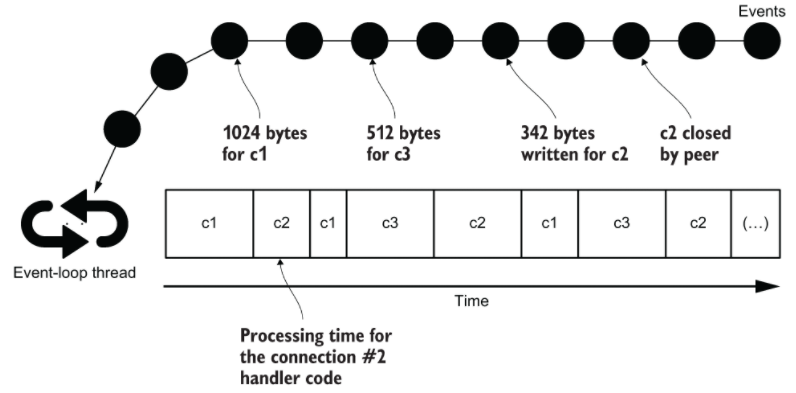
\includegraphics[width=1.0\textwidth]{EventLoop}
	\caption{Exemplarische Abbildung einer Event Loop. \parencite[Kapitel 1.7]{Ponge2020}}
\end{figure}

Dies können beispielsweise I/O-Events sein, die signalisieren das Daten bereit zur Weiterverarbeitung sind, aber auch jegliches andere Event.
Eine Event Loop wird in der Regel auf einem IO-Thread ausgeführt, daher darf das Verarbeiten von Events
keine blockierenden, oder zeitintensiven Operationen beinhalten\parencite{Ponge2020}.

\subsubsection{Quarkus}
\label{section:Quarkus}

Bei dem, in dieser Arbeit verwendeten, Framework Quarkus handelt es sich laut Hersteller Red Hat, um ein
benutzerfreundliches, auf Entwickler abgestimmtes Java Framework, welches für Container-, Cloud- und Serverless-Umgebungen optimiert ist und nur wenig
Konfiguration benötigt, sowie nur die besten und hochwertigsten Java-Bibliotheken und Standards nutzt.
Dabei können die Anwendungen sowohl auf einer JVM (JVM mode) laufen, als auch, durch native Kompilierung mit vollständigem Stack,
als nativ ausführbare Anwendung: dem \textit{native image} (native mode).

Dafür nutzt Quarkus eine, von Oracle entwickelte, Technologie namens GraalVM.
Dabei handelt es sich um eine polyglotte, virtuelle Maschine und Laufzeitumgebung die auf dem OpenJDK basiert, und über
JVMCI \footnote{Java Virtual Machine Compiler Interface} den C2-Compiler der zugrundeliegenden HotSpot-JVM durch den polyglotten Graal JIT-Compiler ersetzt.\parencite{GraalVM}
//TODO genauer erklären wie native image generiert wird, was für anpassugnen an bibliotheken notwendig sind und was der c2 compiler ist und jit compiler

Darüber hinaus verspricht Quarkus mit seiner Container-first-Philosophie, durch \textit{native images} bis zu 300 Mal schnellere Startzeiten
und nur ein Zehntel des
Speicherbedarfs im Vergleich zu traditionellen Java-Frameworks wie Spring Boot, wodurch es eine signifikante Reduzierung der benötigten Ressourcen und Kosten
im Cloud-Umfeld bewirkt. \parencite{RedHatQuarkusInfografik}

Des Weiteren erlaubt Quarkus die Kombination des imperativen und des reaktiven, nicht-blockierenden Programmierparadigmas.
TODO: Vorwärsverweis auf Dispatching von Vert.x auf worker/io thread
Für die reaktive Programmierung bietet Quarkus die bereits genannte Bibliothek Mutiny an.
Quarkus selber ist zudem auch reaktiv, denn es basiert auf der nicht-blockierenden, reaktive Eclipse Vert.x Engine, die
alle Netzwerk I/O-Operationen verarbeitet. \parencite{QuarkusReactiveGettingStarted, Quarkus}

TODO: Noch genauer auf Quarkus eingehen? Erwähnen dass alle Bibliotheken speziell für Quarkus angepasst werden müssen, damit
die native Kompilierung auch funktioniert

TODO: Generell, Entscheidungen mehr begründen (bspw. warum Uber-Jar)